\documentclass{article}

\usepackage[spanish]{babel}
\usepackage[numbers,sort&compress]{natbib}
\usepackage{graphicx}
\usepackage{url}
\usepackage{amsmath}
\usepackage{hyperref}
\usepackage{listings}
\usepackage[top=30mm, bottom=40mm, left=15mm, right=15mm]{geometry}
\usepackage{color}
\usepackage{subfig}
 
\definecolor{codegreen}{rgb}{0,0.6,0}
\definecolor{codegray}{rgb}{0.5,0.5,0.5}
\definecolor{codepurple}{rgb}{0.58,0,0.82}
\definecolor{backcolour}{rgb}{1,1,1}
 
\lstdefinestyle{mystyle}{
    backgroundcolor=\color{backcolour},
    commentstyle=\color{codegreen},
    keywordstyle=\color{magenta},
    numberstyle=\tiny\color{codegray},
    stringstyle=\color{codepurple},
    basicstyle=\footnotesize,
    breakatwhitespace=false,         
    breaklines=true,                 
    captionpos=b,                    
    keepspaces=true,                 
    numbers=left,                    
    numbersep=7pt,                  
    showspaces=false,                
    showstringspaces=false,
    showtabs=false,                  
    tabsize=2
}
 
\lstset{style=mystyle}

\setlength{\parskip}{2mm}
\setlength{\parindent}{0pt}

\author{Edson Raúl Cepeda Márquez}
\title{Autómata Celular}
\date{\today}

\begin{document}

\maketitle

\section{Objetivo}
El objetivo principal de esta práctica es diseñar un experimento en el que se generen células vivas dentro de una malla de 30 por 30 y permita identificar el número de iteraciones que tienen que pasar para que no quede ninguna célula viva dentro de ella. Esta malla representara a nuestro autómata celular. La regla que nos dice cuales células viven y cuales mueren es la siguiente: una célula vivirá si tres de sus vecinos también están vivos, de lo contrario la célula muere.

Se repetira el experimento un determinado número de veces y se variara la probabibilidad con la que aparecen células vivas dentro de la malla para que sea posible analizar los datos con distintas combinaciones de parámetros.

En este reporte se hace uso del código escrito en el lenguaje de programación R \cite{r} que se encuentra en la página \cite{satu} de la Dra. Satu Elisa Schaeffer, así como también el material didáctico de apoyo.

\section{Desarrollo}
El primer paso para diseñar el experimento es comprender las partes más importantes del código y decidir las partes a modificar para cumplir el propósito.

Primero se identfica la variable que nos indica las dimensiones de nuestra malla y se modifica para que ahora las dimensiones sean 30 por 30 :

\lstinputlisting[language = R, firstline = 4, lastline = 4]{P2.R}

Como se trabaja en dos dimensiones, se puede decir que el número de celdas disponibles dentro de la malla es:

\lstinputlisting[language = R, firstline = 5, lastline = 5]{P2.R}

Se procede a especificar la variación de la probabilidad con que las células vivas se generan en la malla:

\lstinputlisting[language = R, firstline = 8, lastline = 8]{P2.R}
\lstinputlisting[language = R, firstline = 11, lastline = 11]{P2.R}

Los casos en que la probabilidad de generar células vivas es igual a 0 e igual a 1 quedan aislados debido a que las distribuciones de células vivas son totalmente uniformes. En probabilidad 0 no se genera ninguna célula y en probabilidad 1 todas las celdas de la malla son ocupadas por células vivas lo cual evita que mueran.

Seguido de esto se especifica el número de repeticiones del experimento:

\lstinputlisting[language = R, firstline = 10, lastline = 10]{P2.R}

Otra de las partes más importantes, es el rango de iteraciones que se realiza para comprobrar la supervivencia de las células en la malla.
En esta parte se debe escoger un número adecuado de iteraciones para poder ver el ciclo de vida de las células sin ninguna limitación.

A continuación se establece un rango de 30 iteraciones, se identifica cuando todas las células ya murieron y se guarda el número de iteración en que lo hicieron:

\lstinputlisting[language = R, firstline = 25, lastline = 42]{P2.R} 

Una vez hecho esto es posible agrupar los datos y graficar los resultados \ref{a}:

\lstinputlisting[language = R, firstline = 39, lastline = 39]{P2.R} 
\lstinputlisting[language = R, firstline = 46, lastline = 46]{P2.R} 

\begin{figure}[h]
\centering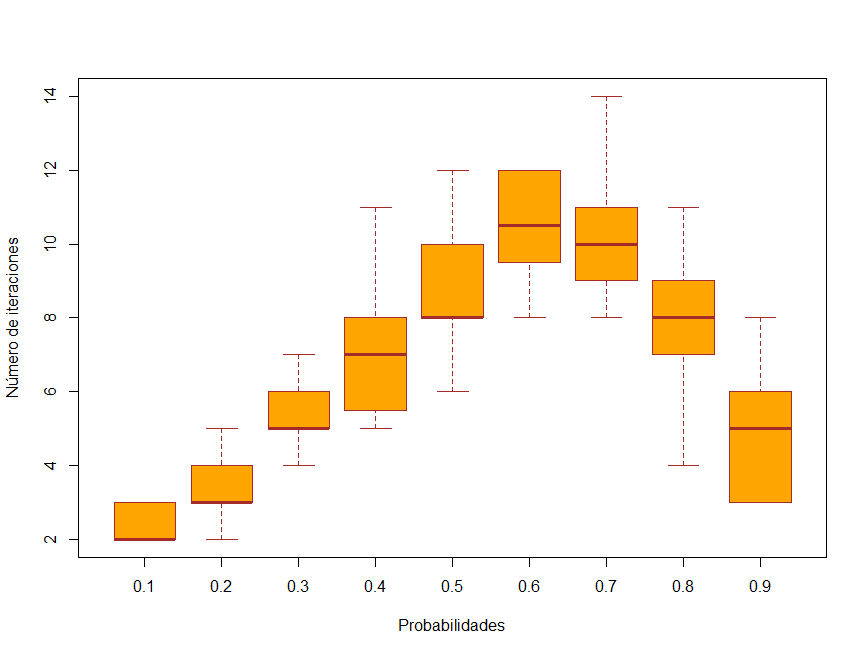
\includegraphics[width = 110mm]{numit.png}
\caption{Número de iteraciones en que murieron las células respecto a su probabilidad de generación.}\label{a}
\end{figure}

Ahora que se han obtenido los resultados, procedemos a analizar los datos y a sacar conclusiones.

\section{Conclusiones}
Analizando los resultados del experimento se observa que, cuantas más células sean generadas, mayor es la duración de la vida de éstas. Cuando la probabilidad de generar células vivas dentro de la malla empieza a tomar valores mayores a 0.4 notamos que el número de iteraciones necesarias para que todas las células mueran empieza a rebasar la cantidad de 10, pero también se puede observar que el número de iteraciones se reduce cuando la probabilidad de generar células vivas toma los valores de 0.7 en adelante.

El número de células que va desapareciendo cuando la probabilidad es muy alta, es mucho mayor que a las anteriores por lo cual las células requieren menos iteraciones para desaparecer, a su vez, podemos observar que en probabilidades entre 0.5 y 0.7 las cosas están equilibradas en el sistema. 

Valores menores a 0.4 hacen que las células en la malla cuenten con menos vecinos lo que hace que todas las células mueran en un tiempo muy corto.

\medskip

\begin{thebibliography}{9}

\bibitem{r} 
R:  R Project, 2019
\\\texttt{https://www.r-project.org/}

\bibitem{satu} 
Satu Elisa Schaeffer: Práctica 2: autómata celular, 2019
\\\texttt{https://elisa.dyndns-web.com/teaching/comp/par/p2.html}


\end{thebibliography}





\end{document}


